\documentclass[10pt,twocolumn]{article}

\usepackage[margin=0.72in,columnsep=0.25in]{geometry}
\usepackage[T1]{fontenc}
\usepackage{newtxtext,newtxmath}
\usepackage{microtype}
\usepackage{amsmath}
\usepackage{booktabs}
\usepackage{graphicx}
\usepackage{xurl}
\usepackage[hidelinks]{hyperref}
\usepackage{flushend}

\setlength{\parindent}{1em}
\setlength{\parskip}{0pt}
\setlength{\textfloatsep}{8pt plus 2pt minus 2pt}
\setlength{\floatsep}{7pt plus 2pt minus 2pt}
\setlength{\abovecaptionskip}{5pt}
\setlength{\belowcaptionskip}{0pt}

\title{\vspace{-1.5em}\textbf{Progressive Photon-Mapping Renderer}\\
\large Implementation and Technical Methods\vspace{-0.4em}}
\author{Parth Gupta\\CS 488}
\date{}

\begin{document}
\maketitle
\vspace{-1.4em}

\begin{abstract}
This report describes a CPU renderer based on the probabilistic progressive
photon-mapping formulation of Knaus and Zwicker ~\cite{knaus2011}  Each iteration first constructs a photon map and then traces camera rays, estimating the radiance at diffuse hitpoints using the photon map and then averaging at the end by the number of iterations. We use the global reference radius method and this radius is reduced according to the equation 15 in ~\cite{knaus2011}. Due to this, no
per-pixel photon counts, flux statistics, or persistent visible points are required.
\end{abstract}

\section{Method Overview}

The renderer estimates global illumination by joining light paths to eye
paths with a local photon-density estimate.  This construction targets light
paths that are difficult to sample by ordinary unidirectional path tracing,
especially paths in which an emitter is seen indirectly through refractive or
reflective surfaces.  The implementation follows the independent-pass,
``memoryless'' progressive photon-mapping (PPM) algorithm of Knaus and Zwicker
\cite{knaus2011}. It is a reformulation of the original progressive photon mapping algorithm of Hachisuka, Ogaki, and Jensen ~\cite{hachisuka2008progressive} and also includes their extension to stochastic progressive photon mapping ~\cite{hachisuka2009stochastic}. The key distinction between this and the original version is that the original one maintains a photon count and accumulated flux at every visible point whereas this one does not store these local statistics.

For iteration $i$, the renderer performs the following operations:

\begin{enumerate}
  \item Trace $M$ paths from the emitters and store every diffuse interaction. This is the photon tracing step and the hitpoints are stored in a kd-tree. 
  \item Trace path from eye until diffuse surfance is hit.
  \item Evaluate radiance with the current
        photon map and radius $r_i$
  \item Add the image to an accumulation buffer and update the radius.
\end{enumerate}

The photon map is discarded before the next iteration.  Thus, memory is linear
in the photons and image pixels of one pass, but independent of the number of
progressive passes.  The final pixel value is the arithmetic mean
\begin{equation}
  \widehat C_N(p)=\frac{1}{N}\sum_{i=1}^{N}\widehat C_i(p),
  \label{eq:pixel-average}
\end{equation}
where each $\widehat C_i$ is evaluated using a newly sampled light distribution
and eye path.  Path throughput accounts for all ideal specular events between
the camera and the first diffuse vertex.

\IfFileExists{sunlit_caustics_bench.png}{%
\begin{figure*}[t]
  \centering
  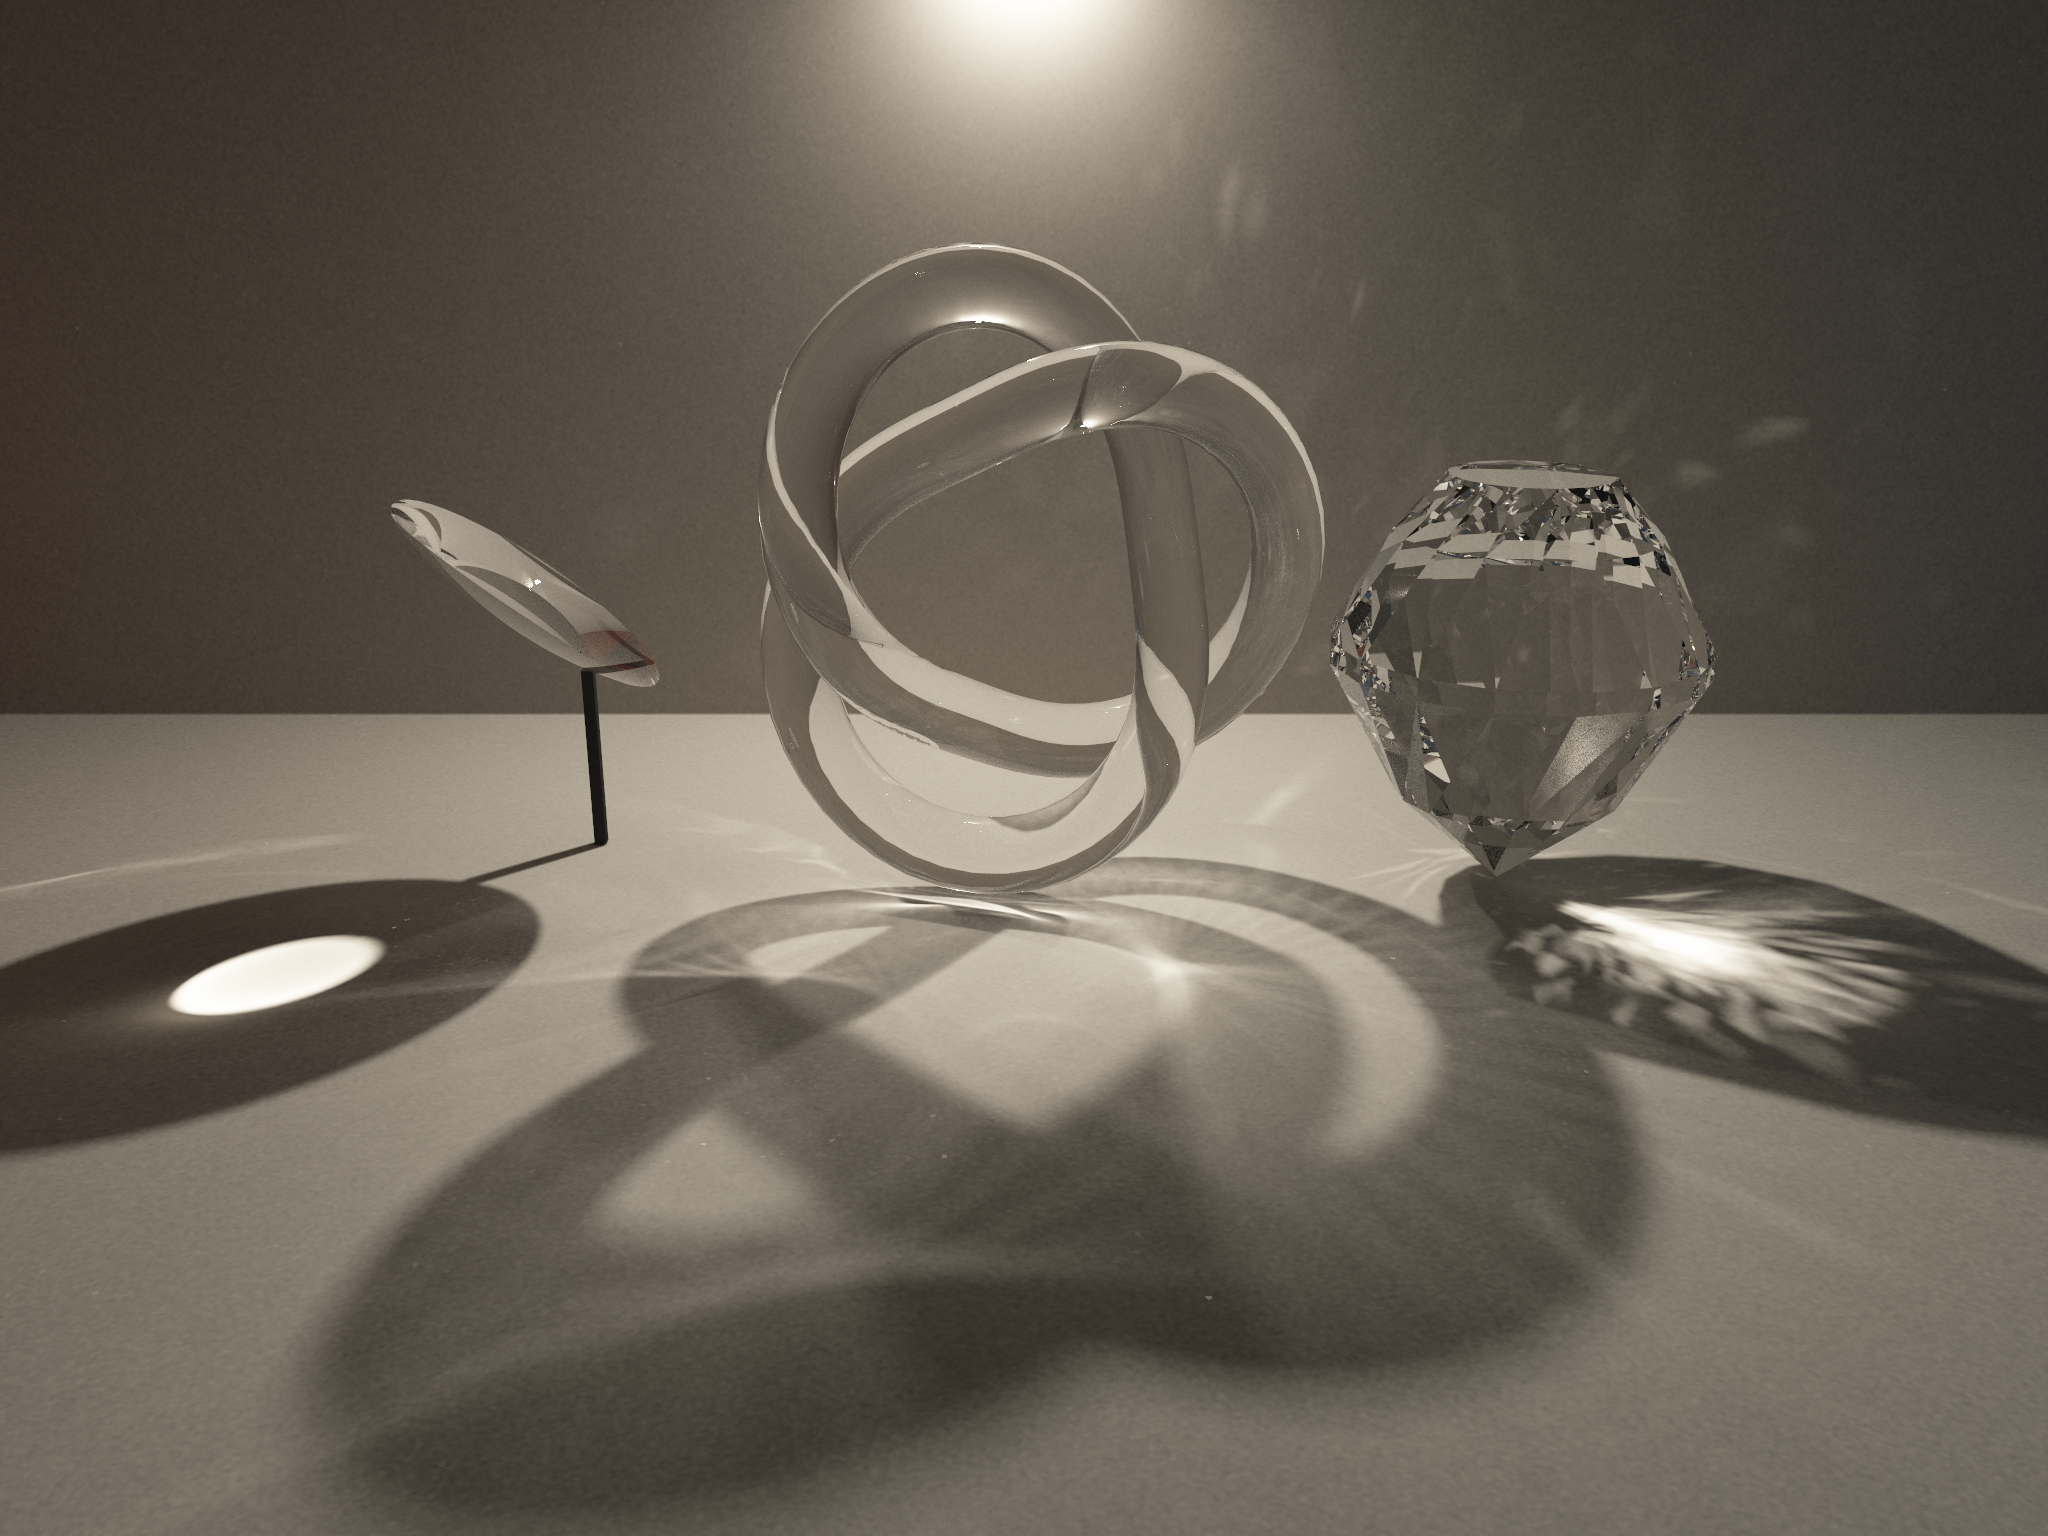
\includegraphics[width=0.82\textwidth,height=0.27\textheight,keepaspectratio]{sunlit_caustics_bench.png}
  \caption{Representative output from the project's caustics scene.  Photon
  density estimation makes focused light transported through the ideal glass
  and mirror geometry directly visible on diffuse receivers.}
  \label{fig:caustics}
\end{figure*}
}{}

\section{Progressive Density Estimation}

At a diffuse surface point $\mathbf{x}$, the implementation uses a uniform box
kernel.  Let $\mathcal{Q}_i(\mathbf{x})$ contain photons in pass $i$ satisfying
\begin{equation}
 \lVert\mathbf{x}_{ij}-\mathbf{x}\rVert < r_i,
 \qquad \boldsymbol\omega_{ij}\!\cdot\!\mathbf{n}>0,
\end{equation}
where $\boldsymbol\omega_{ij}$ is the stored incident direction.  For a
Lambertian material with diffuse reflectance $\mathbf{K}_d$, the outgoing
radiance estimate is
\begin{equation}
 \widehat{\mathbf L}_i(\mathbf{x},\boldsymbol\omega_o)
 = \frac{\mathbf{K}_d}{\pi}
   \frac{1}{M\pi r_i^2}
   \sum_{j\in\mathcal{Q}_i(\mathbf{x})}\boldsymbol\Phi_{ij}.
 \label{eq:density}
\end{equation}
Here $\boldsymbol\Phi_{ij}$ is photon flux and division by $M$ accounts for the
number of emitted primary photon paths.  A single light path may deposit several
photons after successive diffuse bounces, so the number of stored records can
exceed $M$.  All accepted photons receive equal weight. 

The essential progressive step is the global radius update
\begin{equation}
 \frac{r_{i+1}^2}{r_i^2}=\frac{i+\alpha}{i+1},
 \qquad
 r_{i+1}=r_i\sqrt{\frac{i+\alpha}{i+1}},
 \label{eq:radius}
\end{equation}
with $0<\alpha<1$. In the paper, Knaus and Zwicker show that this $\alpha$ determines a tradeoff between vanishing variance and expected value of the average error. The main idea is that the variance is inversely proportional to the square radius and expected error is proportional to the square radius. With some math gymnastics, they are able to show that expected value of the average error goes to $O(1/N^{1-\alpha})$ where $N$ denotes the number of samples of the radiance estimate. Thus, in the limit, we obtain unbiased global illumination. 

\section{Light-Path Sampling}

During scene preprocessing, each triangle whose material has nonzero emission
$\mathbf L_e$ becomes a one-sided area light.  An emitting triangle $\ell$ of
area $A_\ell$ is chosen with probability $p_\ell=A_\ell/A_\Sigma$ where $A_\Sigma$ denotes the total light area.  A position
is sampled uniformly on it using square-root barycentric sampling, and the
initial direction is cosine-weighted over the outward hemisphere,
$p_\omega(\boldsymbol\omega)=\cos\theta/\pi$. The reason for using cosine-weighted sampling is so that directions near the surface normal carry more power as compared to grazing directions.  With
$p_A=1/A_\ell$, the initial photon flux is
\begin{equation}
 \boldsymbol\Phi_0=
 \frac{\mathbf L_e\cos\theta}{p_\ell p_A p_\omega}
 =\frac{\pi A_\ell\mathbf L_e}{p_\ell}
 \label{eq:emission}
\end{equation}

At each surface encounter, a photon is stored before scattering if the material
is diffuse.  The path may then continue, allowing the same map to represent
direct illumination, diffuse interreflection, and caustics. We use a depth limit so that infinitely long path are not taken into account and also use Russian roulette to terminate low-contribution path. Russian roulette
uses the continuation probability
\begin{equation}
 q=\min\!\left(1,\max_c \Phi_c\right)
\end{equation}
and a surviving path has its flux divided by $q$. A limitation here is that bright scenes can cause $q$ to clamp to 1 which defeats its purpose. We used this continuation probability as it was the choice in ~\cite{pbrt}.  The next direction is sampled
from the BSDF, and flux is multiplied by the BSDF, cosine, and inverse PDF.
Light-mode transport also applies an adjoint shading-normal correction and
rejects events for which shading and geometric normals imply inconsistent
hemispheres.

\section{Eye Paths and Materials}

One uniform subpixel sample is generated per pixel in each pass.  A pinhole ray
is traced until it misses the scene, reaches the depth limit, or encounters its
first diffuse surface.  Front-facing emitted radiance is accumulated at every
visited vertex.  At a diffuse hit, Equation~\ref{eq:density} is evaluated and
the eye path terminates.  At an ideal metal or glass hit, a new direction
is sampled and the camera throughput $\boldsymbol\beta$ is updated by
\begin{equation}
 \boldsymbol\beta' = \boldsymbol\beta\,
 \frac{f(\boldsymbol\omega_o,\boldsymbol\omega_i)
       |\boldsymbol\omega_i\cdot\mathbf n_s|}{p(\boldsymbol\omega_i)}.
\end{equation}

The implemented BSDF set is not too involved.  Diffuse materials use
$f_r=\mathbf K_d/\pi$ and cosine-weighted sampling.  Metals are perfect mirrors
scaled by $\mathbf K_s$.  Glass has an index of refraction of
$1.5$ and reflection versus refraction is selected using Schlick's approximation
\begin{equation}
 F(\theta)=F_0+(1-F_0)(1-|\cos\theta|)^5,
 \quad
 F_0=\left(\frac{\eta_i-\eta_t}{\eta_i+\eta_t}\right)^2.
\end{equation}
Snell refraction and total internal reflection are handled explicitly.  The
camera and light passes use separate transport modes so the squared index-of-
refraction factor is applied on the radiance side of transmission.

\section{Spatial Acceleration and Parallelism}

A binary bounding-volume hierarchy (BVH)
accelerates all scene intersections.  Its full-sweep builder evaluates each
triangle-centroid candidate on all three axes using the unnormalized
surface-area cost
\begin{equation}
 C=N_L A_L+N_R A_R,
\end{equation}
and creates leaves containing at most four triangles.  This builder is
quadratic but is performed once before rendering; traversal visits nearer
bounding boxes first.

The photon map is rebuilt in every pass, following the classical spatial
organization of photon mapping \cite{jensen2001}.  It recursively chooses the axis of
largest positional extent and median-partitions photon indices with
\texttt{nth\_element}.  This produces a balanced k-d tree in expected
$O(P\log P)$ build time and $O(P)$ memory for $P$ stored photons.  A radius
query follows the near child and visits the far child only if the query sphere
crosses the splitting plane.  An easy optimization that we do is that the flux is summed during traversal without first
allocating a neighbor list.

We use OpenMP to parallelize expensive independent work.  Photon paths are scheduled
in dynamic blocks of 32, appended to thread-local vectors, and concatenated
before k-d-tree construction.  Camera rows are dynamically distributed one at
a time and write to disjoint pixels.  Each worker owns a persistent 
random-number generator, avoiding synchronization on random sampling.  The
outer progressive loop and both acceleration-structure builds remain serial;
although the probabilistic formulation permits parallel passes in principle,
this implementation parallelizes within each pass.

\IfFileExists{multithreading-mean-performance.png}{%
\begin{figure}[!t]
  \centering
  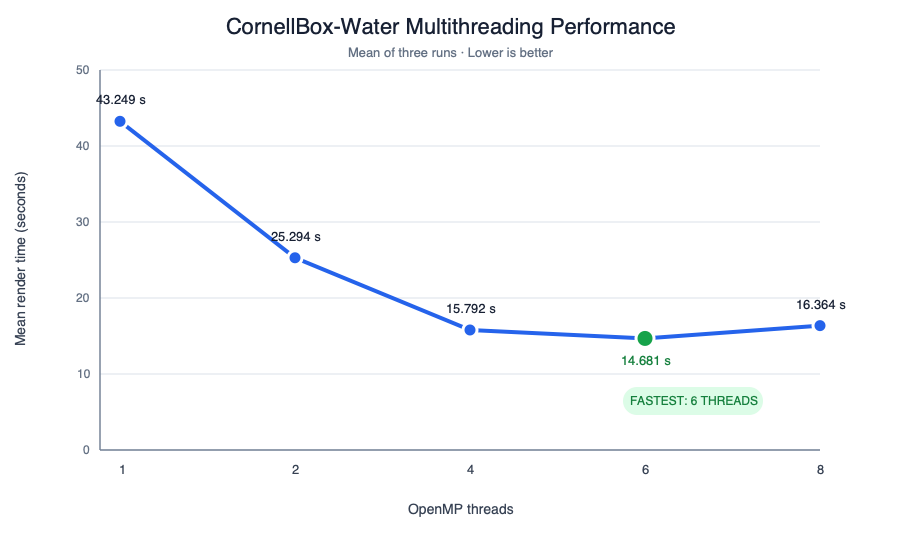
\includegraphics[width=\columnwidth]{multithreading-mean-performance.png}
  \caption{Mean render-only time as a function of the OpenMP thread count for
  the CornellBox-Water scene. Each point is the mean of three runs at
  $512\times384$ resolution with 50 progressive passes, 100,000 photon paths
  per pass, and a maximum path depth of 20. The best measured configuration was
  six threads.}
  \label{fig:multithreading-performance}
\end{figure}
}{}

\begin{table}[t]
\centering
\caption{Current default rendering configuration.}
\label{tab:configuration}
\small
\begin{tabular}{@{}lr@{}}
\toprule
Parameter & Value \\
\midrule
Image resolution & $512\times384$ \\
Vertical field of view & $45^\circ$ \\
Progressive passes $N$ & 50 \\
Photon paths per pass $M$ & 100,000 \\
Eye samples per pixel & 50 total \\
Maximum path depth & 20 \\
Initial radius $r_1$ & 0.02 \\
Radius parameter $\alpha$ & 0.7 \\
Dielectric index $\eta$ & 1.5 \\
\bottomrule
\end{tabular}
\end{table}

\section{Output and Scope}

After all passes, linear RGB is divided by $N$ to account for averaging. We also apply exponential tone mapping given by 
$T(L)=1-\exp[-\max(0,L)]$, followed by a $1/2.2$ gamma curve and 8-bit
PNG quantization. This causes the image to appear more natural as the renders were usually coming out to be very dark due to the hard clamping done previously in the base code.  Table~\ref{tab:configuration} summarizes the current
hard-coded configuration; camera parameters, PPM parameters, and output name
are changed in source rather than through command-line options.

Several restrictions define the estimator's present scope.  The camera is a
pinhole model, materials are limited to Lambertian and ideal delta BSDFs, and
participating media, depth of field, rough reflection, environment lighting,
and explicit direct-light sampling are absent. In addition, material classification uses
project-specific MTL conventions, so input meshes must be triangulated and
prepared accordingly. Also, a robust camera model would be very useful to implement as manually setting camera parameters is cumberson. I would have also really liked to implement some of the stochastic PPM effects like depth of field if I had more time. 



\begin{thebibliography}{9}

\bibitem{knaus2011}
C. Knaus and M. Zwicker,
``Progressive Photon Mapping: A Probabilistic Approach,''
\emph{ACM Transactions on Graphics}, vol. 30, no. 3, article 25, 2011.
\url{https://doi.org/10.1145/1966394.1966404}.

\bibitem{jensen2001}
H. W. Jensen,
``A Practical Guide to Global Illumination Using Photon Maps,''
SIGGRAPH course notes, 2001.
\url{https://graphics.stanford.edu/courses/cs348b-00/course8.pdf}.

\bibitem{pbrt}
M. Pharr, W. Jakob, and G. Humphreys,
\emph{Physically Based Rendering: From Theory to Implementation},
3rd ed. Morgan Kaufmann, 2016.

\bibitem{hachisuka2008progressive}
Toshiya Hachisuka, Shinji Ogaki, and Henrik Wann Jensen.
\newblock Progressive photon mapping.
\newblock \emph{ACM Transactions on Graphics}, 27(5):130:1--130:8, 2008.
\newblock \url{https://doi.org/10.1145/1409060.1409083}.

\bibitem{hachisuka2009stochastic}
Toshiya Hachisuka and Henrik Wann Jensen.
\newblock Stochastic progressive photon mapping.
\newblock \emph{ACM Transactions on Graphics}, 28(5):141:1--141:8, 2009.
\newblock \url{https://doi.org/10.1145/1618452.1618487}.

\end{thebibliography}

\end{document}
